\section{Resolving Ambiguities Using the Abstraction Tree}
\subsection{Resolving Context Ambiguities}
\begin{Verbatim}
function [HM]=eligible(HM_tree,Req)
   BM = all models in HM_tree with all Prop(Req)
	 For all M in BM
	   while (in M no behavior in Prop(Req) is merged with other parameters)
	      M = parent of M
	   endwhile
	 save the parent of M in HM
	 endfor
	 Return HM
\end{Verbatim}

\subsection{Resolving Validity Ambiguities}

\begin{Verbatim}
Input: system model PM, abstraction tree for environment HM_tree, requirement Req
Output: Counter examples CE and corresponding model refinements
[HM]=eligible(HM_tree,Req);
Mc= HM;
    while (Mc is not empty)
		    For all M in Mc
           [satisfied,CE]=ModelChecking(M,PM,Req);
					Remove M from Mc
					If satisfied==0
					    add the children of M to Mc
							cache CE
					else
					  save CE from the parent model
					endif
			endfor
	 endwhile
Return all saved CEs and their corresponding models
\end{Verbatim}



\section{Case Study: }
\label{contextAmbiguities}
\subsection{Requirement Encoding}
\begin{itemize}
	\item Pre-condition: Normal atrial self-activation rate (60bpm - 100bpm)
    \item Post-condition: Ventricular pace rate no faster than LRI
\end{itemize}
\Hao{Need a monitor here}
The requirement can be translated to:
$$R1: NA\_self.min=600,NA\_self.max=1000\Rightarrow VP-VP>=TLRI$$
$Prop(R1)=NA\_self$

$NA\_self$ is in $H_3$, we go one level up, in $H_4$ the behavior is not merged with any other parameters. In $H_5$ $NA\_self$ is merged with  $NA'-NV'.cond$ so $H_4$ is returned as the appropriate heart model for R1. In \cite{STTT13} we used $H_4$ to verify the correctness of the ELT termination algorithm. With a basic DDD pacemaker we have $H_4 || P_{DDD}\models R1$. The counter-example returned is exactly the ELT behavior. Then we implement the ELT termination algorithm and we have  $H_4 || P_{ELT}\not\models R1$, meaning ELT has been successfully terminated, and only the ELT is terminated. 

\subsection{Inappropriate Model Refinements}
If we follow the traditional CEGAR framework and verify the property using $H_5$, an abstract counter-example would return, which is shown in %\figref{C_amiguity}. However the counter-example correspond
 
\begin{figure}[!t]
		\centering
		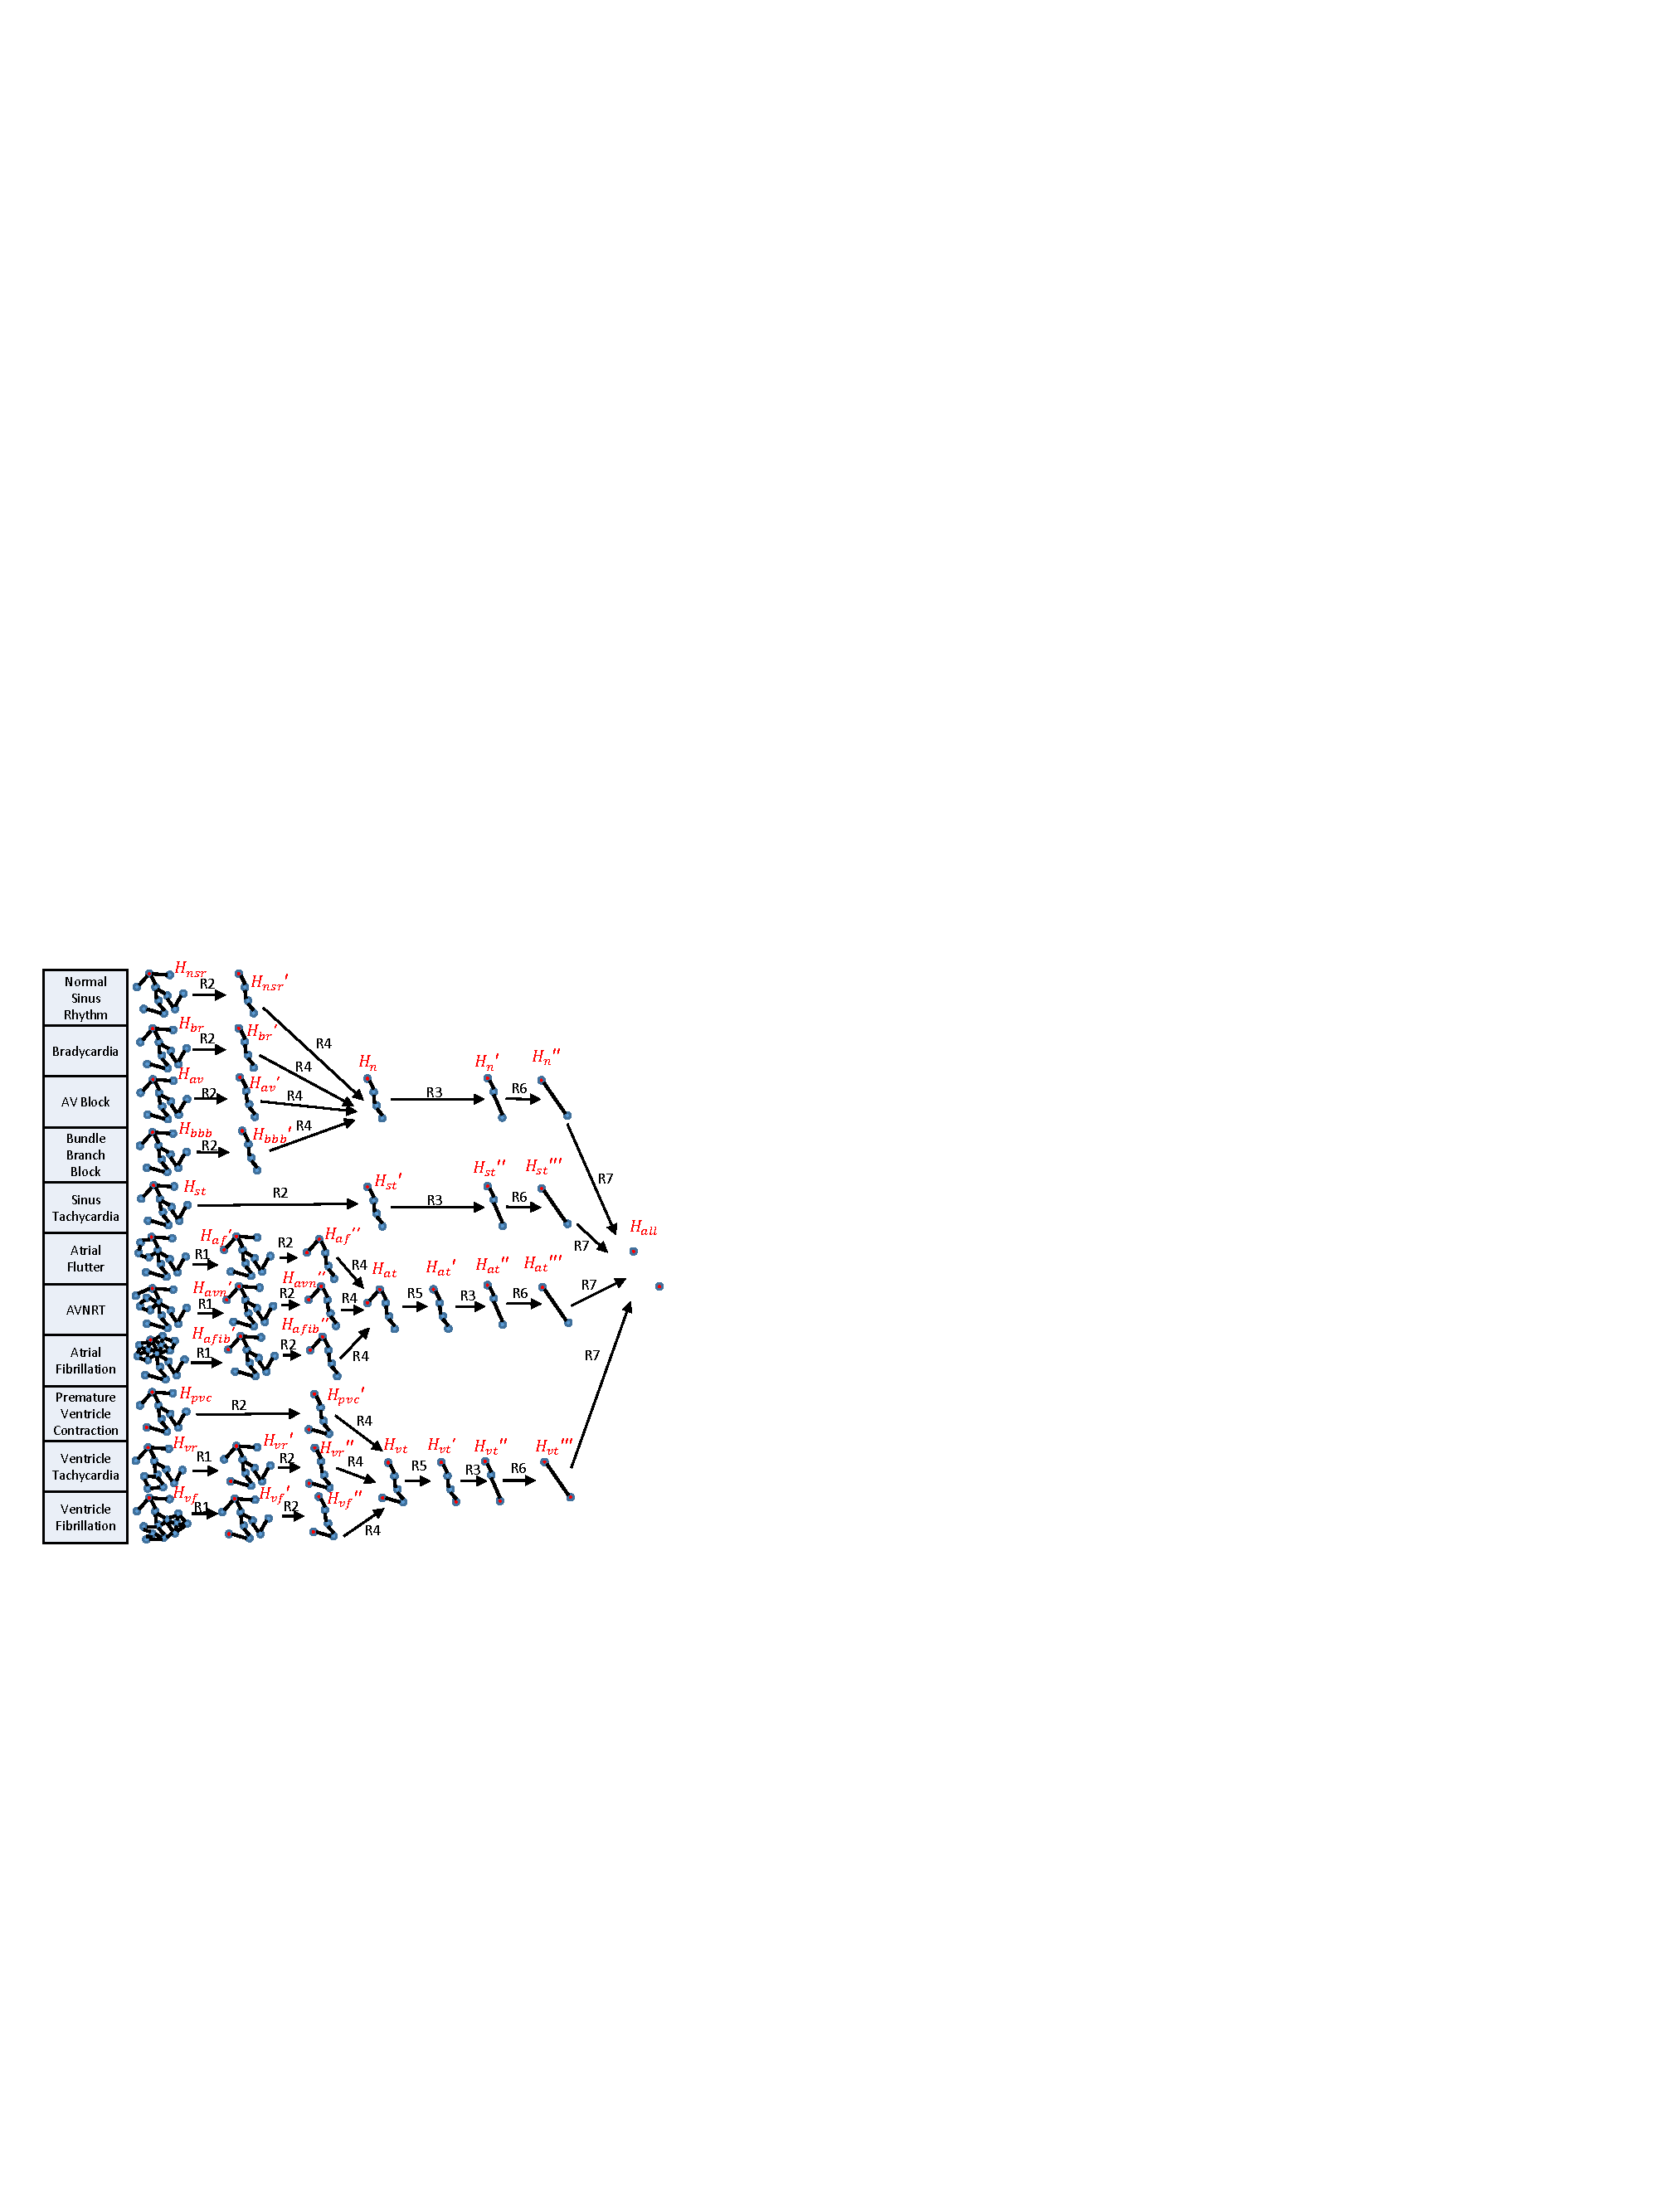
\includegraphics[width=0.9\textwidth]{figs/abs.pdf}
		%\vspace{-5pt}
		\caption{\small Heart Model Abstractions}
		  %\vspace{-15pt}
		\label{fig:HM_abs}
\end{figure}



